\subsection{Preprocesamiento De Los Datos} 
Con el objetivo de darle mayor estabilidad matematica a los datos y quitar algo del ruido que puedan tener, realizamos un preprocesamiento de los mismos. Este consistió en quitar los utliers dentro de nuestras muestras y luego normalizarlos con media 0 y varianza 1.

\subsection{Implementacion Del algoritmo} 

El algoritmo que implementamos consistio en una red neuronal profunda con retropropagación del error. El algoritmo descripto de manera informal consiste en introducir una instancia del problema, calcular la salida, compararla con la salida esperada y retropropagar el error, con el objetivo modificar las matrices de pesos y minimizar la diferencia. El sistema implementado se dice ser $online$ ya que los pesos de las matrices son ajutados luego de retropropagar el error de cada instancia en vez de hacerlo al final de la epoca.

A fin de tener una medida de como va "aprendiendo" la red neuronal, luego de mostrarle todas las instancias una vez, calculamos la norma del error de todas las instancias para saber cuanto nos acercamos o nos alejamos de la solución ideal.

%habria que poner pseudocodigo o algo mas lindo acá
Aprovechando este calculo de la norma, decidimos agregar a la implementación, un learning rate adaptativo. El mismo consiste en, en caso de que la norma haya decrecido, aumentar el learnin rate. En caso contrario, es decir, la norma del error aumentó, quiere decir que la red empeoro la solucion y decrecemos el learnig rate.

Como optimización adicional se agrego un termino de momentum. La idea tras esto consiste en darle a cada peso de la matriz una "inercia" que le permita continuar avanzando en la direccion en la que avanzó en la iteración anterior. El objetivo consiste en disminuir las oscilaciones con cada pequeño cambio en la matriz.

\subsection{Performance Diagnostico de Cancer} 

Para este problema utilizaremos una neurona en la ulima capa con función de activación $tanh$. Para ser consistentes con esto, las salidas esperadas adoptarán los valores 1 si resulto ser cancer maligno, y -1.0 si resulto ser benigno. La experimentación consistirá en buscar los parametros optimos que nos den la mayor tasa de aciertos para nuestro data set.

Como primera instancia buscamos cual era la cantidad optima de neuronas necesarias para la resolución del problema, fijamos el learning rate en $0.01$ y el momentum en $0.9$, y fijamos para una capa oculta, graficamos los datos obtenidos:

\begin{figure}[!ht]
  \centering
    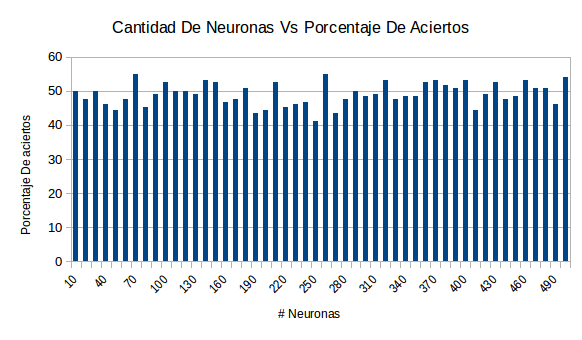
\includegraphics[scale=0.5]{neruonas_vs_aciertos.png}
\end{figure}

El modelo no parece adaptar mejor para una mayor cantidad de neuronas, seteamos la cantidad de neuronas en $70$ ya que ahí parece alcanzar el mejor valor.

Luego variamos el learning rate, dejando todos los otros parametros como antes, lo obtenido puede verse en el siguiente grafico:

\begin{figure}[!ht]
  \centering
    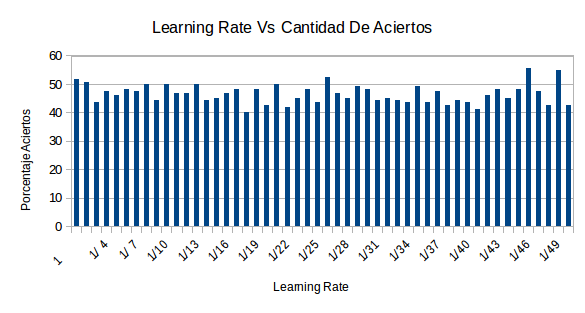
\includegraphics[scale=0.5]{learning_rate.png}
\end{figure}

En el grafico puede obsercarse que para un learning rate de $1/	46$ parece haber un maximo en la cantidad de aciertos de $55\%$ . Luego nos quedamos con este valor.

%completar
Despues learning rate, y momentum

\subsection{Performance Regreción Lineal Calor} 

%falta implementar
Por cuestiones de tiempo este ejercicio no fue probado de manera adecuada